\documentclass[a4paper]{report}
\usepackage{amsmath,graphicx,tikz}
\usepackage{makecourse}
\usetikzlibrary[topaths]
\newcount\mycount

\begin{document}
\setcounter{chapter}{1}
\chapter{A chapter title}

\section{Figures}
\subsection{Graphics}
\begin{figure}
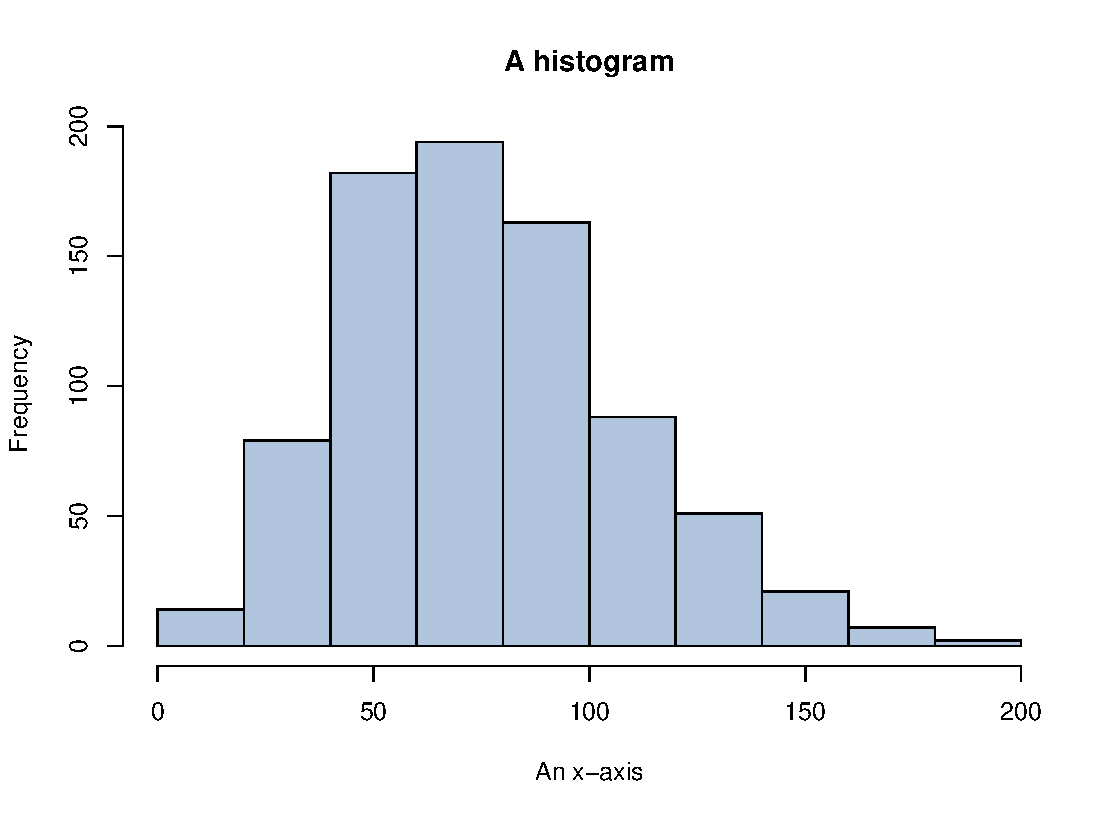
\includegraphics[width=0.8\textwidth]{images/hist.pdf}
\caption{A histogram originally provided in .pdf format}
\alttext{A plot titled "A histogram". The x axis is labelled "x-axis".
	The y axis is labelled "Frequency". The histogram shows a peak at
	a value of approximately 70.}
\end{figure}

\subsection{Tikz}
% A complete graph
% Author: Quintin Jean-Noël
% <http://moais.imag.fr/membres/jean-noel.quintin/>
\begin{figure}
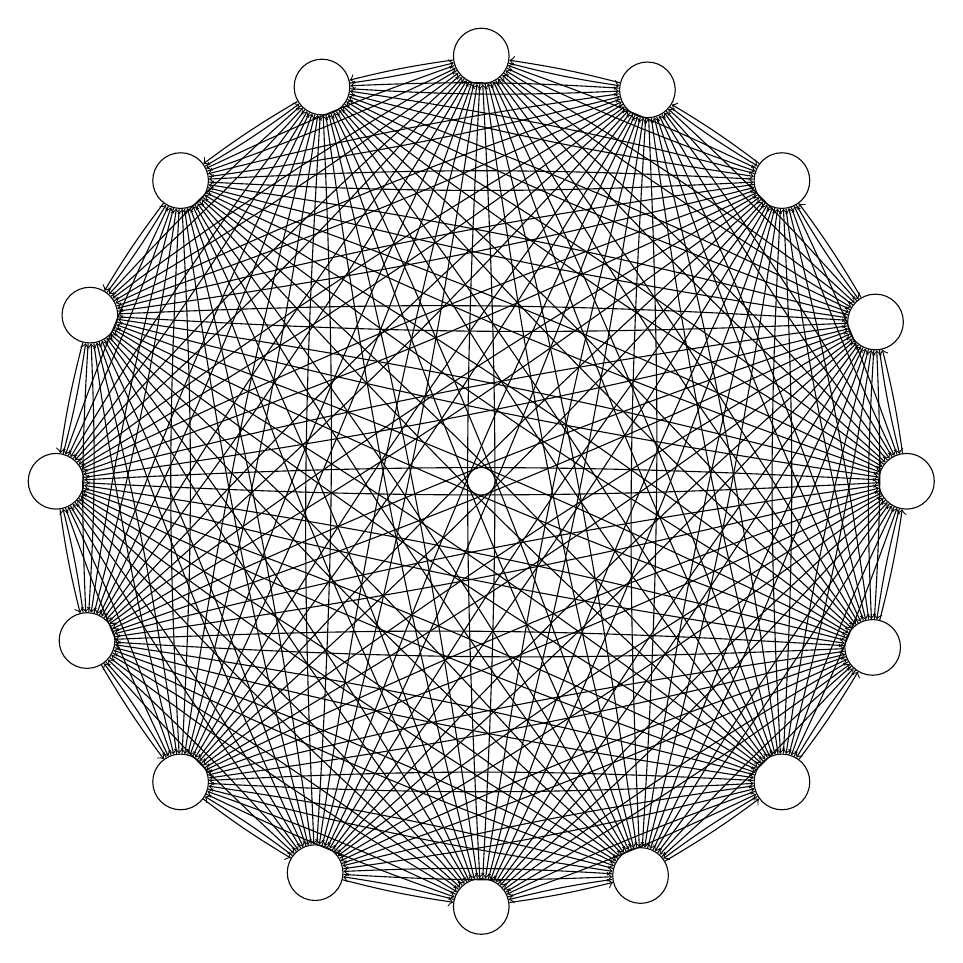
\begin{tikzpicture}[transform shape]
  \foreach \number in {1,...,8}{
        \mycount=\number
        \advance\mycount by -1
  \multiply\mycount by 45
        \advance\mycount by 0
      \node[draw,circle,inner sep=0.25cm] (N-\number) at (\the\mycount:5.4cm) {};
    }
  \foreach \number in {9,...,16}{
        \mycount=\number
        \advance\mycount by -1
  \multiply\mycount by 45
        \advance\mycount by 22.5
      \node[draw,circle,inner sep=0.25cm] (N-\number) at (\the\mycount:5.4cm) {};
    }
  \foreach \number in {1,...,15}{
        \mycount=\number
        \advance\mycount by 1
  \foreach \numbera in {\the\mycount,...,16}{
    \path (N-\number) edge[->,bend right=3] (N-\numbera)  edge[<-,bend
      left=3] (N-\numbera);
  }
}
\end{tikzpicture}
\caption{A complete graph, drawn with tikz.}
\alttext{A \textbf{tikz} figure showing a graph with 16 nodes. Each node is connected to every other node.}
\end{figure}

\section{Embedding}
\subsection{Numbas}
\numbas{https://numbas.mathcentre.ac.uk/test-yourself/maths-support-diagnostic-test-differentiation/}
\subsection{Vimeo}
\vimeo{8169375}
\subsection{Youtube}
\youtube{EdyociU35u8}

\end{document}
